\chapter{工程选址分析}
\label{chp:location:begin}
\section{火星地形分析}

\subsection{火星地形分布概况}

火星上的地形地貌种类相对于地球较少,大部分的区域被沙漠和戈壁覆盖,两极被冰层覆盖,中间零星穿插着高地、山脉、峡谷和裂谷。另外,火星由于靠近小行星带,遭受的陨石撞击较多,所以也有很多的陨石坑。

\subsection{火星主要地形分析}

1、沙漠平原:

1)基本情况:沙漠在火星上占了较大的比例,除两极外均有较广泛的分布,沙丘也将其他的地形阻挡开来,对地形之间的转移造成不便。

2)气候:沙丘上均有沙尘暴,沙尘暴持续时间较短,强度较大。

3)灾害:沙尘暴掩埋。

4)原位资源:长期的沙尘暴气候使得可利用的地下资源除于深度掩埋和随机掩埋的状态,难以寻找和利用。

5)舱体固定:沙漠地区的地质结构松散,舱体不便固定,只能选择大体积的组装舱或者充气舱,防止被沙尘暴吹走。除此之外,平原上的建筑不宜过高。

2、戈壁滩:

1)基本情况:戈壁滩在火星上成片分布,总面积小于沙漠覆盖面积,戈壁滩地形较为稳固,少数地面偶有充满甲烷的孔洞。

2)气候:戈壁滩的沙尘暴强度弱于沙丘,持续时间更短。

3)灾害:除沙尘暴之外,在孔洞附近可能发生火灾或者爆炸。孔洞也可能引起地质沉降。

4)原位资源:固态铁矿、甲烷孔洞内的甲烷。

5)舱体固定:固态岩石使得在戈壁滩上建造有地基的建筑成为可能,若是建造有地基的建筑,就可以将不同功能的建筑分散,防止意外发生时成片影响。但是由于孔洞的存在,可能会有不稳定的地质活动。

\begin{figure}[H]
  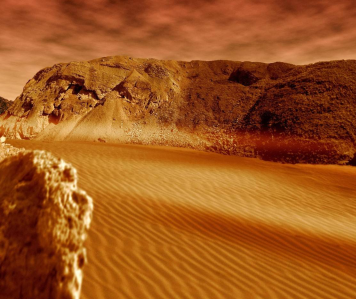
\includegraphics[width=0.8\textwidth]{figure/shamo-gebi.png}
  \centering
  \caption{火星的沙漠和戈壁}
\end{figure}


3、高地和火山:

1)基本情况:火星上有很多的山脉,除开部分可能除于活动的火山之外,大多数山脉的海拔就较高,最高的超过 21000米。拿火星上的奥林帕斯山举例,它的占地面积超过英国国土面积,坡度非常平缓,山体附近有许多裂纹,预计其附近的地质活动会比较剧烈。

2)气候:高地可以阻挡沙尘暴等自然灾害。

3)灾害:由于火星重力较低,山体附近的地质活动可能比较剧烈,驻地附近可能会出现裂缝等。

4)原位资源:山体(尤其是部分火山)附近的甲烷含量会比较高,部分火山附近也有较多的甲烷孔洞,山体和山体附近具有较多的地热能(火星地壳较薄)溢出,对于能源的采集可能会有利。

5)舱体固定:山体的固态岩石有利于建筑的固定,但是由于地质活动较为强烈,可能建筑体积不能太大,并且要易于迁移。

\begin{figure}[H]
  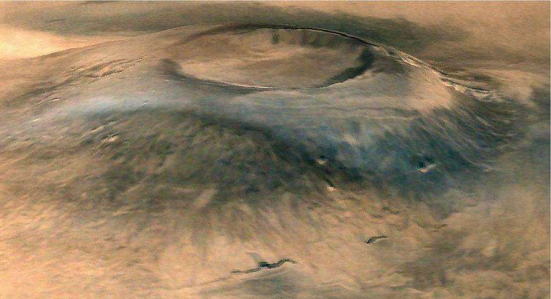
\includegraphics[width=0.8\textwidth]{figure/huoshan.png}
  \centering
  \caption{火星上的火山}
\end{figure}


4、两极冰盖及附近:

1)基本情况:火星两极的冰盖主要由干冰和水冰构成,呈现交互叠加的状态,每层的冰盖较薄。

2)气候:平均气温较低,有因自转因素形成的微弱气旋。

3)灾害:冰层较薄且混有干冰,导致地质不稳定。

4)原位资源:干冰和水冰可采,太阳能视季节可能不充足。

5)舱体固定:不稳定的地形导致舱体无法在冰盖上直接固定(干冰受基地热源影响易挥发导致地质沉降),放置舱体的位置考虑选择在地形交接处(即冰盖的边缘固态岩石地区)。

\begin{figure}[H]
  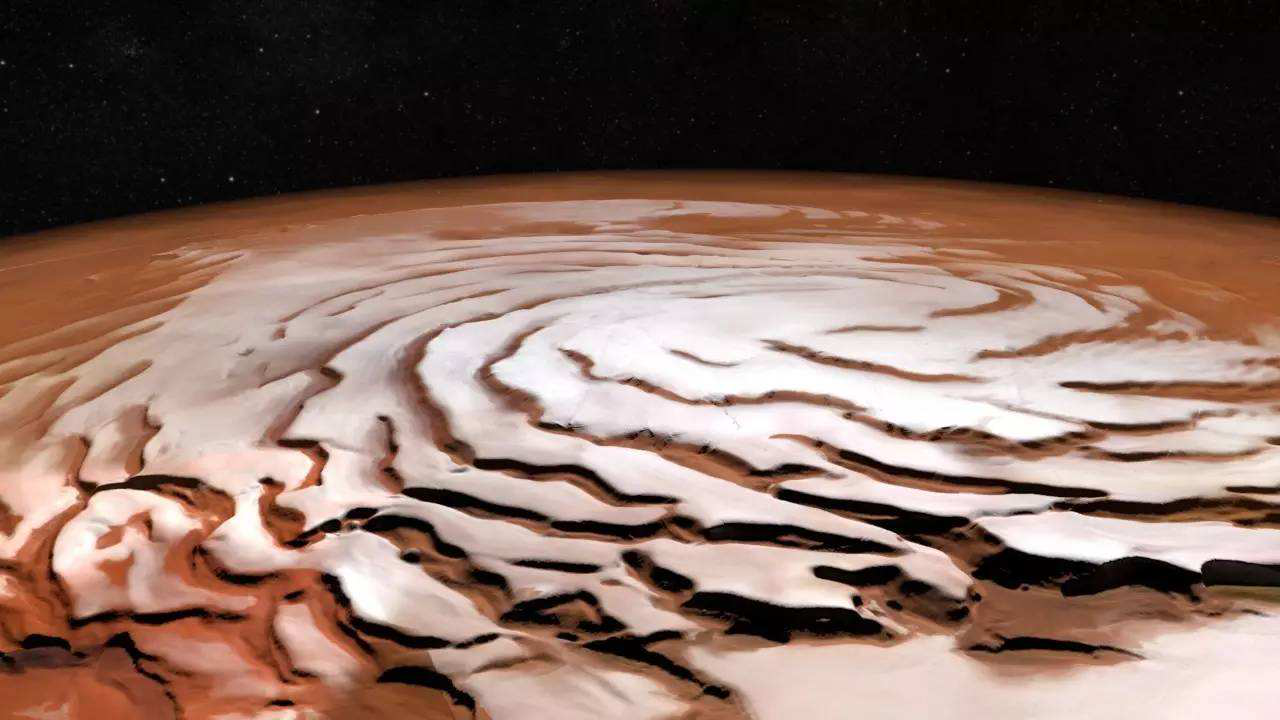
\includegraphics[width=0.8\textwidth]{figure/binggai.png}
  \centering
  \caption{两极冰盖}
\end{figure}


5、峡谷和裂谷:

1)基本情况:火星上有一些峡谷,形成原因比较多样,包括地表侵蚀(水侵蚀、冰川侵蚀、火山活动引起的侵蚀)和地质活动。根据峡谷的成因不同,峡谷的情况可能差别较大,\cref{tab:location-xiagu} 列举了三种裂谷的差异。

\begin{table}[H]
  \centering
  \caption{三种成因形成的峡谷对比}
  \label{tab:location-xiagu}
  \begin{tabular}{|>{\centering}m{0.15\textwidth}|>{\centering}m{0.2\textwidth}|m{0.5\textwidth}|}
    \hline
    \multirow{2}{=}{水侵蚀和冰川侵蚀} & 灾害 & 地质活动相对于其他裂谷可能更少,强度也会更弱。\tabularnewline
    \cline{2-3}
    & 原位资源 & 侵蚀点附近可能有较易采集的地下水和地下冰川资源(包括水冰和干冰)。\tabularnewline

    \hline
    \multirow{2}{=}{火山活动引起的侵蚀} & 灾害 & 处于火山附近,地质活动更剧烈,遭遇火山活动等情况时难以逃脱。\tabularnewline
    \cline{2-3}
    & 原位资源 &  附近空气中的甲烷含量会比较高,部分火山附近也有较多的甲烷孔洞,附近有较多的地热能溢出,对于能源的采集可能会有利。\tabularnewline

    \hline
    \multirow{2}{=}{地质活动形成的裂谷} & 灾害 & 地质结构不稳定,地质活动非常剧烈,不可预测。\tabularnewline
    \cline{2-3}
    & 原位资源 & 地壳较薄,可能采集更多的地下水、地下甲烷等资源,可利用一些地热能。 \tabularnewline
    \hline
  \end{tabular}
\end{table}

2)气候和灾害:舱体置于峡谷中可阻挡沙尘暴(但峡谷太窄会有被掩埋的风险)。峡谷是地质不稳定地带,根据成因会有不同的地质灾害。

3)舱体固定:峡谷内部属于地壳薄弱区域,加上火星本身的地壳就比较薄,所以在峡谷内部固定舱体可能会有较大的风险。

\begin{figure}[H]
  \centering
  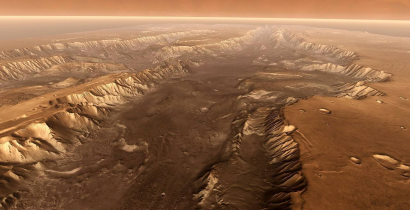
\includegraphics[width=0.8\textwidth]{figure/xiagu.png}
  \caption{水和冰川侵蚀形成的峡谷}
\end{figure}

6、陨石坑:

1)基本情况:火星上有一些陨石坑,较大的陨石坑可以形成盆地地形。陨石坑的分布比较随机,但稳定的陨石坑基本都处于固态岩石的地段。

2)灾害:陨石坑可以较好地阻挡沙尘暴的灾害。但较小的陨石坑有遭沙尘暴掩埋的风险。

3)原位资源:陨石坑的分布较为随机,没有固定的原位资源可供利用。较大较深的陨石坑破坏了更多的地壳,可能会较易采集到地下资源(包括地下甲烷、地下水、地下干冰等),更易利用到地热能。

\begin{figure}[H]
  \centering
  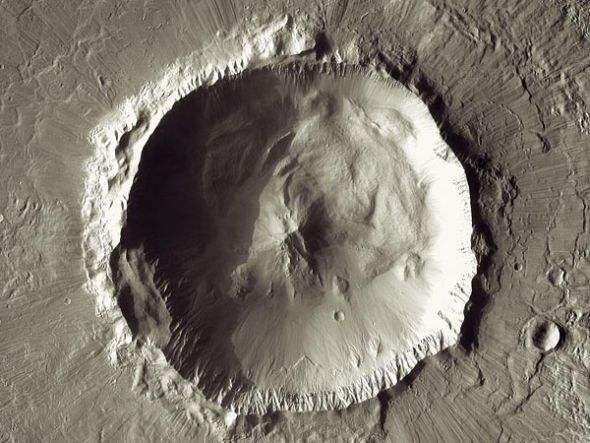
\includegraphics[width=0.6\textwidth]{figure/yunshikeng.png}
  \caption{火星上的陨石坑}
\end{figure}

7、火山坑:

1)基本情况:火山坑是巨型火山的遗迹,规模最大的火山坑有 1200平方公里,深度有1750米深。火星上完全活跃的火山不多,大多数的火山坑是处于不活动的状态。由于火星重力较低,火山坑的平均海拔要比地球上高。

2)气候:火山坑的平均深度深于陨石坑(此结论源于对多个固态星球分析的结果,并非对火星单一的结论),考虑到火星火山的平均高海拔,火山坑内部的气压应该略低于地表气压,但由于火星的大气压非常小,所以气压的差异影响不会很大。除此之外,外界的气候对于火山坑内部几乎没有影响。

3)灾害:火山坑最大的自然灾害威胁便是其活跃的地质结构和有害气体。火山坑内也有非常多的孔洞,会涌出含硫的有毒气体。

4)原位资源:丰富也易于采集和保存的地热能,火山坑内的平均气温也远高于地表平均气温,有丰富的甲烷、硫化氢等气体可采集。

5) 舱体固定:活跃的地形会导致舱体的固定出现一些困难,由于受到外界气温的影响较小,可以考虑不建设地基,直接放置舱段。

\begin{figure}[H]
  \centering
  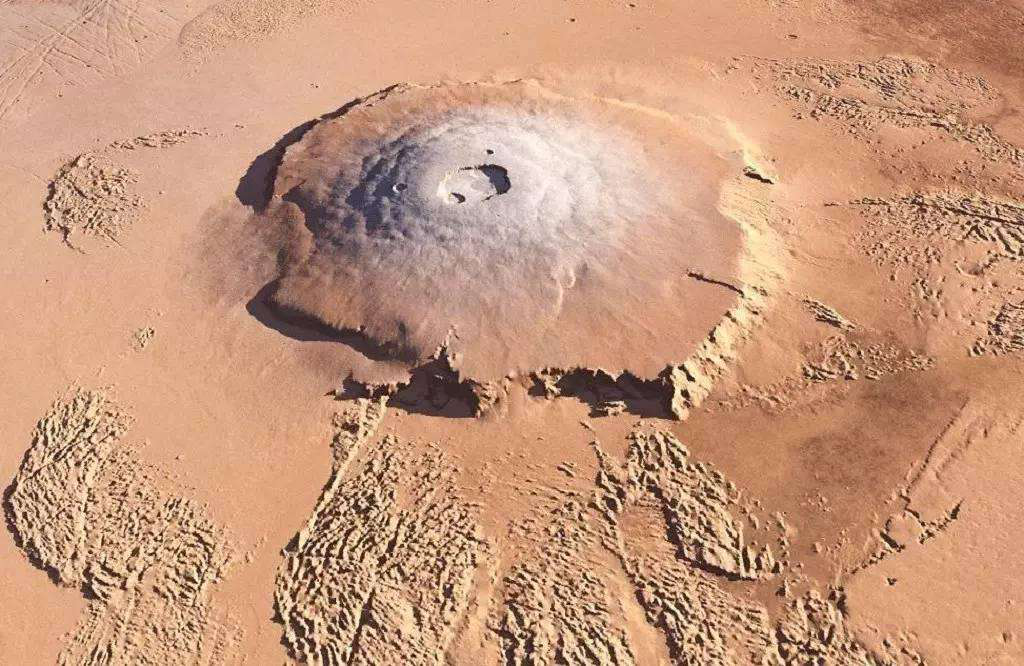
\includegraphics[width=0.8\textwidth]{figure/huoshankeng.png}
  \caption{奥林匹斯盾形火山及其火山坑}
\end{figure}

\subsection{地形分析总结}

通过以上的分析,可以看出不同的地形是各有优劣的。总体来讲,沙漠是最平凡的地形,但几乎没有可利用的资源,不适合用于长期基地的建设,戈壁滩也有类似的问题。因此首先排除这两种地形。在剩下的地形里考虑选址。

\section{基地选址确定}

1、通过讨论和分析,我们决定将选址定在北纬25°附近火山坑道,选择此纬度是因为火星对应位置的风沙强度较小。标准的坑道尺寸拟定如下:

1)面积:600平方公里(最大火山坑道面积的一半)

2)深度:1000米

3)海拔高度:4000米(以坑底为基准)

4)地质活跃度:低

5)平均气温:5--10\si{\degreeCelsius}

6)舱体位置:距离坑道边缘5公里处

7)边缘升降装置:4个,等距离分布在舱体附近的坑道边缘
\vskip1cm
\begin{figure}[H]
  \centering
  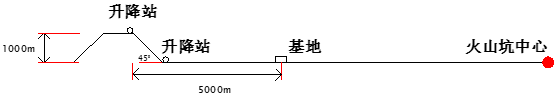
\includegraphics[width=\textwidth]{figure/location-sideview.png}
  \caption{选址剖视图}
\end{figure}

\begin{figure}[H]
\label{chp:location:end}
  \centering
  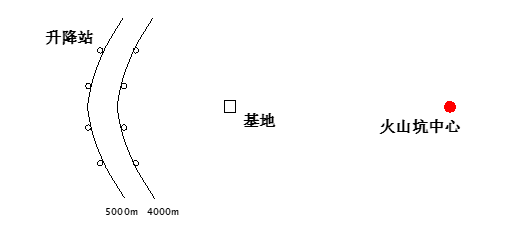
\includegraphics[width=\textwidth]{figure/location-topview.png}
  \caption{选址俯视图}
\end{figure}

2、选址的理由:

1)远高于地表的平均温度:就算是地质活跃度低的火山坑,其内部的平均温度也是远高于地表温度的,受到昼夜因素的影响也较小,非常有利于舱体的保温。

2)最丰富的地热能:火山坑是所有可用地形中利用地热能机会最大的,并且其可利用的地热能也是最丰富的,采集也是最为容易的。这一点我们会在舱体设计和能源采集中体现。

3)高海拔和坑道深度阻碍外界灾害:火山坑的分布特点决定了其几乎不受外界沙尘暴和气旋的影响。除了有害气体和可能的地质活动,火山坑没有其他灾害影响。但是在舱体设计方面,我们仍然会考虑舱体的除尘效果。
